\documentclass[letterpaper,11pt,twocolumn]{article}
\usepackage{fullpage}
\usepackage{color}
\usepackage{graphicx}
\usepackage{epsfig}
\usepackage{amsthm}
\usepackage{latexsym}
\usepackage{amssymb}
\usepackage{amsmath}

\newcommand{\newfontobj}[2]{
  \newcommand{#1}[1]{
    \expandafter\def\csname##1\endcsname{{#2 ##1}}}}

\newfontobj{\class}{\rm} % Typeset Classes in roman font

% Some standard classes (use in only mathmode)
% Usage example: $\P \subseteq \NP$ and we believe that $\NP$ is not equal to $\P$.

\class{PSPACE}
\class{L}
\class{BPL}
\class{RL}
\class{NC}
\class{ZPL}
\class{NPSPACE}
\class{ASPACE}
\class{NL}
\class{EXP}
\class{NEXP}
\class{coNEXP}
\class{NE}
\class{E}
\class{AM}
\class{MA}
\class{NP}
\class{DNP}
\class{UP}
\class{P}
\class{RP}
\class{BPP}
\class{ZPP}
\class{EXPSPACE}
\class{coNP}
\class{coRP}
\class{coAM}
\class{PH}
\class{IP}
\class{PCP}
\class{MIP}
\class{SE}

% operator classes.
\class{BP}

% these commands should be used in math mode - $ $
\newcommand{\SHARPP}{{\#\rm{P}}}
\newcommand{\PARITYP}{{\oplus\rm{P}}}

% math operators...
\DeclareMathOperator{\poly}{poly}
\DeclareMathOperator{\Majority}{Majority}
\DeclareMathOperator{\quasipoly}{quasi-poly}
\DeclareMathOperator{\polylog}{poly-log}
\DeclareMathOperator{\superpoly}{super-poly}
\DeclareMathOperator{\DTISP}{DTISP}
\DeclareMathOperator{\DSPACE}{DSPACE}
\DeclareMathOperator{\DTIME}{DTIME}
\DeclareMathOperator{\NSPACE}{NSPACE}
\DeclareMathOperator{\NTIME}{NTIME}
\DeclareMathOperator{\BPTIME}{BPTIME}
\DeclareMathOperator{\RTIME}{RTIME}
\DeclareMathOperator{\ZPTIME}{ZPTIME}
\DeclareMathOperator{\BPSPACE}{BPSPACE}
\DeclareMathOperator{\RSPACE}{RSPACE}
\DeclareMathOperator{\ZPSPACE}{ZPSPACE}
\DeclareMathOperator{\med}{med}


% Complexity class
\newcommand{\CC}{\mathcal{C}}


% add DRAFT to your document %
\newcommand{\draft}[0]{
\begin{center}
	{\bf \Large {\sc DRAFT} }
\end{center}
}

% example environment
\newenvironment{example}
{\smallskip \noindent \emph{Example:}}
{\hfill $\boxtimes$ \smallskip}

% some theorem environments
\newtheorem{conjecture}{Conjecture}
\newtheorem{theorem}{Theorem}
\newtheorem{proposition}{Proposition}
\newtheorem{claim}{Claim}
\newtheorem{lemma}{Lemma}
\newtheorem{corollary}{Corollary}
\newtheorem{definition}{Definition} % Use this for non-trivial
	% definitions.

% currently not used %
\newtheorem{exercise}{Exercise}
\newtheoremstyle{example}{\topsep}{\topsep}%
     {\normalfont \small}   % Body font
     {}    % Indent amount (empty = no indent, \parindent = para indent)
     {\bfseries}     % Thm head font
     {}%           Punctuation after thm head
     {\topsep}%     Space after thm head
     {}%         Thm head spec    \theoremstyle{example}
\theoremstyle{example}
%\newtheorem{example}{Example}

\usepackage{multicol}
\usepackage{fullpage}
\usepackage{url}
\usepackage[top=1in, bottom=1in, left=1in, right=1in]{geometry}
\usepackage{hyperref}
\usepackage{multirow}
\usepackage{enumerate}
\pagenumbering{arabic}
\setlength{\columnsep}{0.25in}

\title{\bf{MicroswiftOS : A Minimal OS for Cloud Computing}}
\author{
  Menghui Wang\\
  Department of Computer Sciences\\
  \texttt{menghui@cs.wisc.edu}
  \and
  Yiran Wang\\
  Department of Computer Sciences\\
  \texttt{yiran@cs.wisc.edu}
  \and
  Chaowen Yu\\
  Department of Computer Sciences\\
  \texttt{ycw@cs.wisc.edu}
  \and
  Junhan Zhu\\
  Electrical and Computer Engineering\\
  \texttt{jzhu84@wisc.edu}
}
\date{May 3, 2015}
\begin{document}
\twocolumn[
\maketitle
\draft
]
\begin{abstract}
Infrastructure as a service (IaaS) is a popular cloud computing model where each customer will get access to a virtual machine running on the data center hosted by the service provider. Compared to traditional options, IaaS is a more reliable and economy solution when it comes to web hosting, cloud computing, data storage, or other workloads. Such cloud applications have different demands than a traditional program running on a personal computer - such as high availabilities, and ease to migration. MicroswiftOS, a specialized OS for cloud applications running in virtual machines, is built to best meet these requirements. It features a much faster boot-up time and a lightweight system size to enable high availability for applications and a more efficient storage for host machines. Experiments show our MicroswiftOS has met both goals.
\end{abstract}

% \begin{multicols}{2}
%\category{B.3.2}{Hardware}{Memory Structure\----\textit{Cache Memories}}

%\terms{}

%\keywords{}

\section{Introduction}
\label{sec:intro}
Cloud computing launches a new era of computer systems - new service models, such as Infrastructure as a Service (IaaS), providing computing resources for customers to deploy their own applications. This brings new challenges to both ends of the cloud: for software applications, it is worth deliberating how to migrate multi-tier applications to provide scalable and reliable services \cite{zheng2014comma}; for operating systems hosting client applications, there is much room for optimizations to achieve smaller system size as well as better performance. Since IaaS providers often offer virtual machines rather than physical ones, quite a few features that a regular operation system provides become unnecessary or unimportant, which leaves us opportunities for optimizations.

In modern data centers, a cloud infrastructure usually consists of many physical host machines, each hosts a various number of guest virtual machines where user applications reside. Such infrastructure is widely adopted, because it helps cloud service providers make best use of their hardware resources, comparing to the alternative where a set of dedicated hardware is provided to each user. The use of virtual machines opens the door for guest OS optimization: (1) Hardware related features are hardly useful in the guest operating system, for it is only running on virtual machines - for instance, support for hot-pluggable device is never useful on a cloud virtual machine. (2) Cloud service providers would like to cut down the size of guest operating systems for storage efficiency. (3) Smaller-sized operating systems are easier to migrate to another physical machine, taking less time and bandwidth. (4) With refined analysis and careful investigation into the kernel modules, removing or modifying certain parts of the OS would not do harm to its performance.

\begin{figure}[!htb]
\centering
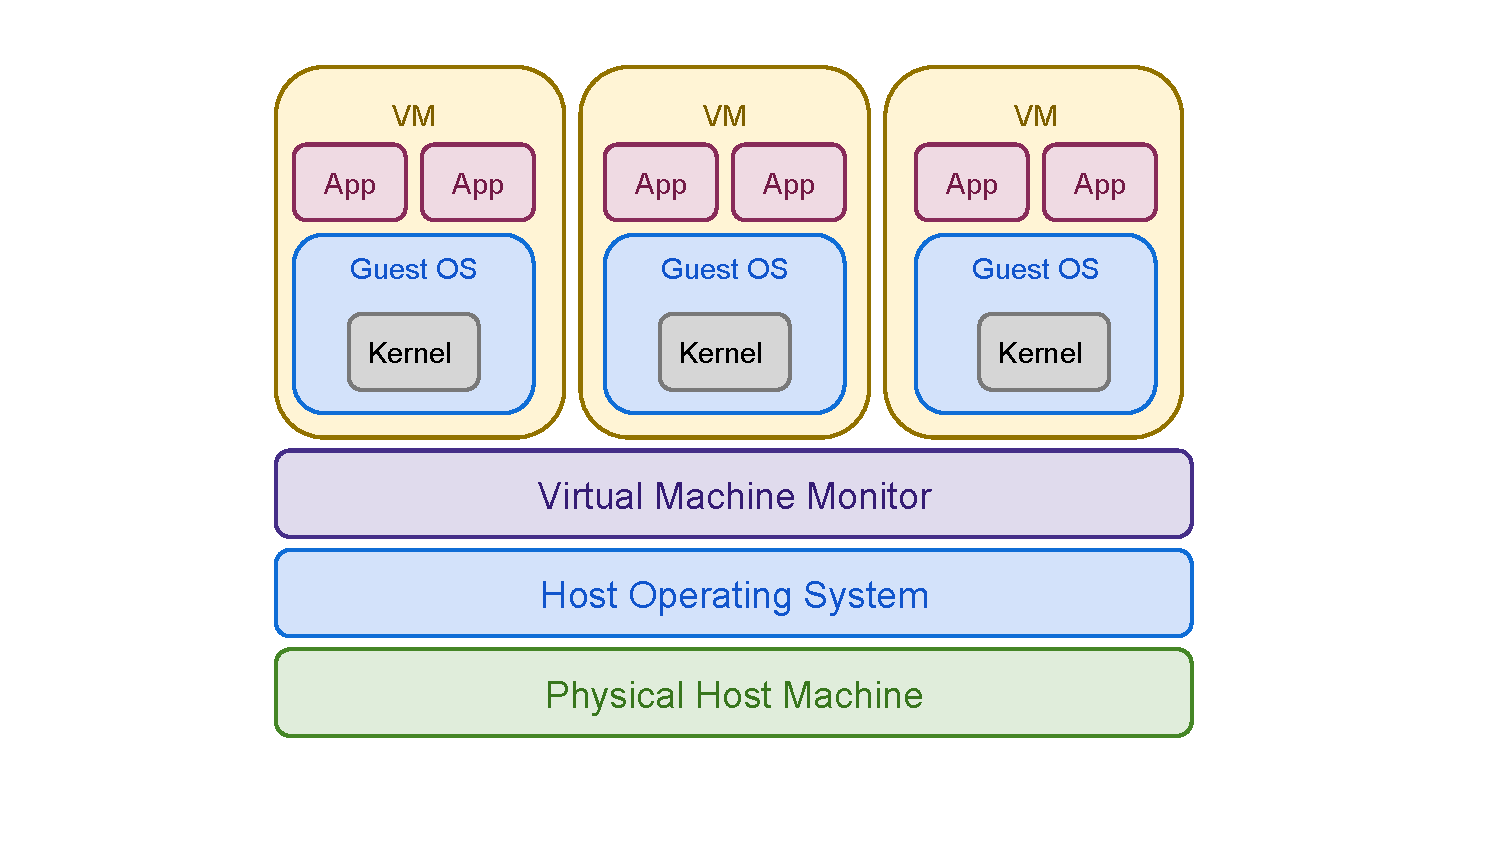
\includegraphics[width=3.4in]{graphs.pdf}
\caption{\label{fig:structure}MicroswiftOS structure}
\end{figure}

In this project, we try to minimize the Linux operating system to accommodate the requirements of a user machine in cloud. In particular, we aim at guest operating systems running in virtual machines, since most cloud service providers today would give their customers virtual machines that they have complete controls over. 

Moreover, the guest operating system could be optimized to support the hosted applications in achieving better availability and performance \cite{fox2009above}. For most applications deployed on the cloud, one of the major issues that operations staff care about is the average downtime. In practice, application downtime is inevitable due to (1) preventive system maintenance, (2) application install or upgrade deployment, (3) application failures or outages. In each case, a large amount of time is spent on operating system booting up or rebooting. Therefore, it is important to shorten OS boot-up time to help improve application availability. There are some methods already discovered to speed up Linux booting - disabling unnecessary kernel modules, using a text-based login instead of a graphical login, etc. With a rapid-boot system, our cloud users are able to bring their applications back alive shortly after they experienced a program failure or finished new deployment.

In this project, we make an effort to speed things up during system boot time besides minimizing the size of a regular Linux system. Our goal is to tailor the Linux operating system to the needs of a guest OS running on virtual machines in the cloud, and to optimize the micro-OS for swift boot-up. We test our minimal OS for essential features that support common user applications in cloud, such as a simple web server, a scientific computing task, and basic communication services etc. \cite{iosup2011performance}

The rest of this paper is structured as follows. Section \ref{sec:moti} captures the characteristics of a kernel running in a cloud, explaining why kernel minimization is feasible and plausible. Section \ref{sec:micro} analyzes how we managed to strip down the kernel and obtain MicroswiftOS. It covers several aspects from kernel configurations to boot script optimizations. The implementation details are in Section \ref{sec:impl}. And Section \ref{sec:eval} summarizes the evaluation of MicroswiftOS including system speed, system size and system completeness. Section \ref{sec:related} introduces several interesting papers related to our work. Finally Section \ref{sec:future} concludes our paper with some future work. We also include appendices to summarize experiment results, provide detailed information on evaluation, elaborate on how we obtain the testing data, and justify the fairness and credibility of our evaluation.

\section{Motivations}
\label{sec:moti}

Nowadays, an increasing number of companies and individuals choose to use infrastructure as a service (IaaS) platforms to host their applications, such as Amazon AWS, Microsoft Azure, and Google Cloud Platform to accomplish various tasks including web serving, scientific computations, data storage, application request handling, etc.
IaaS customers usually have access to a virtual machine hosted on a physical machine owned by the service provider. Customers can choose their favorite operating system from a preset list, which usually includes some popular Linux distributions and Windows, and they will be able to get full privilege in the operating system they have chosen. Compared to using their own hardwares, IaaS provides customers with a more reliable, flexible, and cost-efficient solution.

Workloads carried out on the cloud have their special characteristics that are different from ordinary workloads expected on a personal computer.One of major characteristics is that a virtual machine on the cloud is usually dedicated to one certain task, such as web serving. Various tasks are deployed on different virtual machines, providing separation between applications. When one application encounters a fault, we can easily recover the error by restarting the application or the virtual machine without interfering other running applications.

Secondly, the availability of the applications matters. Customers who pay for public cloud service usually come to this decision as they care about the jobs running on the cloud, and would like to seek better support for high availability. Some user applications, such as the web server of a popular online shopping site, may cause huge profit loss if they are unavailable for a period of time. 

Thirdly, applications on the cloud do not care about hardware-related features provided by the OS. Cloud service customers do not have physical access to the machine hosting their applications. Therefore certain operations would never take place in IaaS scenarios, such as installing new hardware, or inserting a USB flash key. In addition, as applications will always run on top of a virtual machine, the OS chosen by the customer does not have real control over the hardware of the host machine, but only sees virtualized hardware presented by the Virtual machine monitor.

All of these bring up new opportunities for us to optimize the guest operating systems running in virtual machines to better serve the purposes of the workloads.
We want to build a specialized operating system to use in cloud computing with shorter boot-up time and smaller size, and it still meets the requirements of applications running on top of it.

\subsection{Swift Boot-up}
The availability of an application is calculated by
$$\frac{MTTF}{MTTF+MTTR}$$
where $MTTF$ is mean time to failure for the service and $MTTR$ is mean time to repair the failed service. When a failure occurs, usually the time spent on rebooting the system contributes a big portion of $MTTR$. This is especially true when certain monitoring services are deployed, in which they can monitor and detect failures, and in case a failure happens, it promptly reboots the failed machine. Therefore reducing the boot-up time of the OS can help increase the availability of applications running in the cloud.

There are a lot of opportunities for us to optimize the boot-up time. For instance, users and applications on the cloud are less interested in hardware-related functionalities, such as device management and disk utilities. Many modules and can be removed from the kernel, e.g., RAMDisk.

\subsection{Minimized OS Size}
There are two major benefits of minimizing the size of the guest OS. Firstly, since a physical machine in the cloud will usually hosts many virtual machines, we will be able to save a lot of space if we are able to cut down the size of each guest OS a little. Second, a minimized OS size also enables more efficient migration because of the reduced transmission cost from one physical machine to another.

Since most virtual machine will only run one specific task, rarely an application will need a wide collection of software, as provided by most Linux distributions. Even though, MicroswiftOS still provides a complete toolchain to users to build and install software, so that when a software in need is not included by default, the user will be able to add it to the system manually.

\section{Analysis and Methodologies}
\label{sec:micro}

MicroswiftOS is an operating system based on Linux and it is optimized for use in cloud computing. It is designed to run on virtual machines. It features fast boot-up and a relatively small image size.

\subsection{Optimizing Kernel Configurations}

The OS kernel of MicroswiftOS is Linux 3.19, though various changes have been made to it in an effort to speed up booting and shrink kernel size. The kernel features a full-fledged configuration and many modules that could be conveniently added on, but most of these features are not used in cloud computing at all. For example, the guest operating system mainly focuses on computing and does not resort to all kinds of peripherals. Some related features such as all-inclusive file system support could be disabled. Some debugging features such as early printk could also be disabled as once our guest OS starts service we assume it does not suffer substantial debugging. Kernel modules could be completely removed because in a cloud computing environment most kinds of services are predefined and ad-hoc functionality changes should not occur. These features and functionalities can be configured before compiling the kernel thus we can prevent the corresponding code from being compiled in the first place.
Our first attempt is to find a minimal set of features to be involved in the compiling phase that guarantees successful system start up and shut down. By manipulating these configurations, we find a list of features that could be disabled in addition to those already being disabled in default configuration, see Appendix A.

To understand the behavior of operating system boot-up, we use perf - a commonly used statistical profiler in Linux - to collect sample data on the execution of a User-mode Linux (UML) and to conduct dynamic program analysis \cite{perf2013}. Since we mainly care about the activities happening at system booting, we use perf to profile a process that does the following tasks:
\begin{enumerate}[(1)]
\item Boot UML;
\item Log in Linux;
\item Halt
\end{enumerate}
We use FlameGraph to visualize the profiling reports - the x-axis spans the sample population, sorted alphabetically, and the y-axis shows stack depth. The function beneath a function is its parent, just like a stack traceback. The first graph is generated from the sample data collected by perf while we execute User-mode Linux with default configurations; and the second graph is generated from that of a minimized UML kernel. When we try to analyze the profiling data we have collected, we encountered a problem of missing symbols and we have not yet figured it out till now. Therefore some of the samples are only reported with their memory addresses instead of commands in the graphs above. But we can still gain some insights from their overall behaviors: for instance, with default configurations the Linux system spends a large amount of time working on something unsymbolized, as shown at the left most part of the graph; while the minimized UML kernel does not have a corresponding timespan. 

\subsection{Optimizing System Configurations and Software Environments}

Apart from the kernel, an operating system will also need a software environment to run. Pre-installed softwares and configurations will serve for a number of important purposes: 
\begin{enumerate}
\item
Providing a file system on a partitioned disk that the OS will mount as root. The file system will need to conform to the Filesystem Hierarchy Standard of Linux, which requires it to have a various number of pre-created folders such as /bin, /lib, etc.
\item
Bootstrapping the OS. This includes boot-loading the kernel, instructing the kernel on how to mount the root file system and what kernel modules to load and where they are located, and providing an init program that the kernel will run after booting has completed.
\item
Providing a shell program in which user can enter commands and read outputs.
\item
Providing handy tools utilities that users can use to execute common tasks and build softwares, such as a compiler, binary utilities, headers for system APIs, libraries, text editors, manuals and documentations, etc. Though theoretically this part is optional, it is usually highly recommended.
\end{enumerate}

Most popular Linux distributions have configured their system to best meet the needs of an ordinary PC user. On the contrary, we configured MicroswiftOS to best meet the requirements of cloud-hosted applications. 

\subsubsection{Optimize Boot Scripts}
After the kernel boots up, a startup script starts to run to do initialization work, such as setting run levels, mounting file systems, and initializing kernel modules, etc. We can modify some parts in this scripts to speed up the booting process. For example, we can disable the module used for supporting hot-pluggable devices because users will not have physical contacts with the host machine. As a second example, at a certain step the script will wait for udev (a device manager for Linux kernel) initializations to complete before executing the next steps. This is necessary when subsequent initialization steps will use udev; however this is not the case for MicroswiftOS, so we can make subsequent steps to start as soon as possible.

\subsubsection{Disable initramfs}
initramfs was a mechanism introduced to simplify the booting process. During booting a lot of components such as file systems, disks, device drivers, need to be initialized.
However the resources and configurations that are needed to initialize these components are stored in the file system on disk, therefore it brings the problem of egg and chicken. initramfs is a compressed file system image that includes all essential files needed to initialize the system. If initramfs is enabled, the boot loader will first loaded it directly into the memory, and that the kernel can boot with all essential tools ready. Initramfs simplifies the booting process a lot when the file system or device layout is rather complicated.

We decide to disable initramfs because loading the ramfs into memory takes too much time. Besides, initramfs provides no actual benefit for cloud computing. This is because the disk layout is usually simple for virtual machines, and users are not expected to change any device related configures.

\subsubsection{Disable fsck On Boot}

Under default settings each partition will need to be checked using fsck before mounted at boot. This is mainly to detect disk corruptions. Since MicroSwiftOS is designed to run in a virtual machine, the disks it sees are actually files residing in the host OS. As a result, fsck would not be necessary because the host file system will be responsible for integrity checks and providing correct files.

\subsubsection{A Minimal Software Collection and a Complete Toolchain}
MicroswiftOS includes everything needed to build a software: a compiler, a linker, a library loader, a text editor, bash utilities, common libraries, debugging tools, manuals and documents. On the other hand, it does not include more software than that. User will need to build and install any softwares that they need to run their application. This will not be a big hassle, because cloud virtual machines will usually be dedicated to only one task, and as a result the virtual machines will only need to be configured once.

\section{Implementation}
\label{sec:impl}

We constructed MicroswiftOS from scratch. The general procedures were similar to what was listed on Linux from Scratch \cite{beekmans1999linux}, except that a few packages were removed and certain configurations were changed. We choose not to describe every detail as it was a tedious procedure and the exact details can be found online. Instead, we will only highlight general ideas and things we have changed.

\subsection{Building a Temporary System}

A temporary system will include some basic tools that we need to build every software in MicroswiftOS, like gcc, glibc, binutils, etc.
The reason we cannot use tools in the current system is to make sure nothing will be built for the current platform or be linked with libraries in the current system.

\subsection{Building Softwares and Tools}

Using the tools in the temporary system, we will compile and install every piece of software we need.
For a complete list of software installed on MicroswiftOS, check Appendix D.

\subsection{Building the Kernel}
The linux kernel is compiled using the configuration detected in the previous section. Besides, the �Virtualization� option must be selected.

\subsection{Changing Certain Configuration Files}
\begin{enumerate}
\item
Change the grub configuration file properly so that grub will boot MicroswiftOS.
\item
Get rid of the "initrd" line in the grub configuration file to disable ramdisk.
\item
Add "loglevel=4" to the kernel command-line arguments so as to decrease the number of messages being logged. This would also slightly speed up the booting process \cite{bird2004methods}.
\item
Change /etc/fstab to disable fsck for the root partition.
\item
Change /etc/sysconfig/rc.site so as to disable wait for udev\_settle.
\end{enumerate}

\subsection{Cleanup and Reboot}
Remove temporary files used to build system and reboot.

\section{Evaluation}
\label{sec:eval}
\subsection{Environment}
We installed MicroswiftOS as a virtual machine instance in Virtualbox 4.3.8, configured to have 4GB virtualized memory and a single processor. It was running on a host computer with processor Intel I3-4130 (3.4GHz, dual core), 8GB physical memory. The host OS was Windows 7. We also installed an instance of Archlinux in Virtualbox as a comparson OS. We have chosen Archlinux as our comparison OS because compared to Gentoo or Ubuntu, it provides a relatively clean and lightweight system after installation.
\subsection{System Completeness}

In this section we show that MicroswiftOS is able to build and run normal Linux programs correctly with no performance loss. We selected a wide range of workloads to represent the actual cloud computing use cases: thttpd, a selection of some classic algorithms, a benchmark for interprocess communications.

thttpd is an open-source lightweight web server which has a compact code base while delivering superior performance. We have installed thttpd on MicroswiftOS and made it serve a simple HTML page. Then we used another computer to open that web page, and the web page shown was correct. This demonstrates that MicroswiftOS is able to run network-related workloads correctly.

We have also prepared a set of programs that run some classic algorithms: the push-relabel algorithm to solve the maximum flow problem, the Gaussian-Jordan elimination algorithm to solve linear systems, the simplex algorithm to solve linear programmings. We grabbed the code of these algorithms from a code library used for competitive programming contest - this is to say, these implementations have been verified to be correct. We tried to build and run these algorithms on MicroswiftOS under a set of randomly generated input data. Integer arithmetics were covered in the data for max flow, and floating point arithmetics were covered in the data for the linear system solver and the simplex solver. For a detailed description of how input data were generated, see Appendix. We then verified its correctness by comparing its output with the output generated by another computer. No errors were found. These algorithm represents a category of scientific computation workloads, and our test has shown that MicroswiftOS is able to run scientific workloads correctly.

We also benchmarked the performance of inter-process communication on MicroswiftOS, as was conducted in a previous mini-project \cite{mini}. Specifically, we measured the latency and throughput of MicroswiftOS, through $3$ different inter-process communication mechanisms: pipe, socket, mmap. We also did the same measurement for Archlinux as our control group. Results are shown on Figure \ref{figure:latency} and Figure \ref{figure:throughput}. From the results we learn that the IPC performance of MicroswiftOS and Archlinux are comparable.

\subsection{Boot-up Time}

We measured the boot-up times of the system under $3$ different configurations: an original Archlinux as baseline, Archlinux's kernel with the image of MicroswiftOS, and MicroswiftOS's kernel with MicroswiftOS's image. \footnote{Originally we also planned to measure the boot time of MicroswiftOS's kernel with Archlinux's image, but it seems that the Archlinux image requires certain kernel configuration options to be selected when compiling the kernel, or otherwise it won't boot.
We was not able to figure it out at the end.} Boot-up times were measured using a stopwatch between the point when a GRUB menu item is selected and the appearance of the login prompt.

Results are shown on Figure \ref{figure:eval}. From the results we know that both our kernel optimizations and image optimizations are effective, with image optimizations being more effective than kernel optimizations, and overall they cut down the boot-up time by half compared to the baseline system.

\begin{figure}[!htb]
\centering
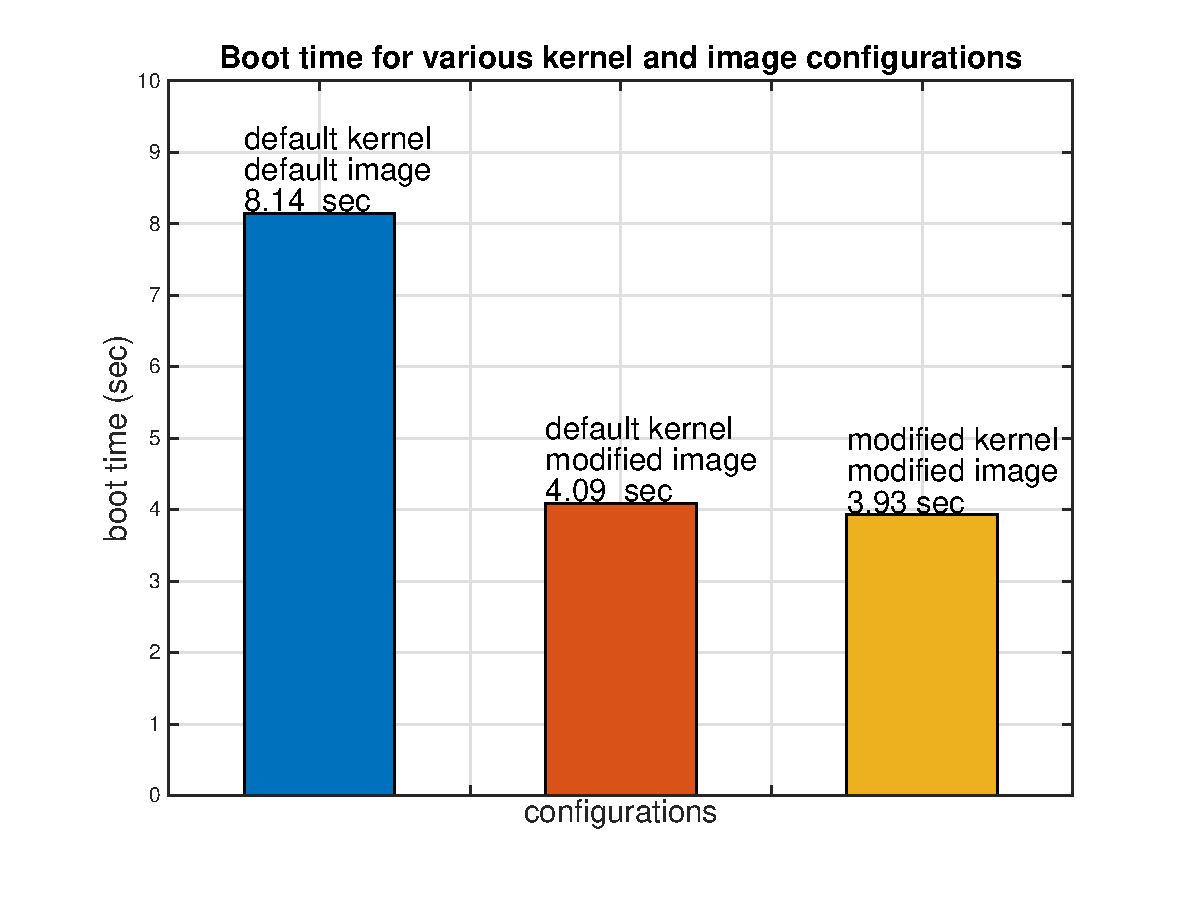
\epsfig{file=evaluation.eps, width=3.4in}
\caption{Boot-up time for various configurations}
\label{figure:eval}
\end{figure}

\begin{figure*}[!htb]
\centering
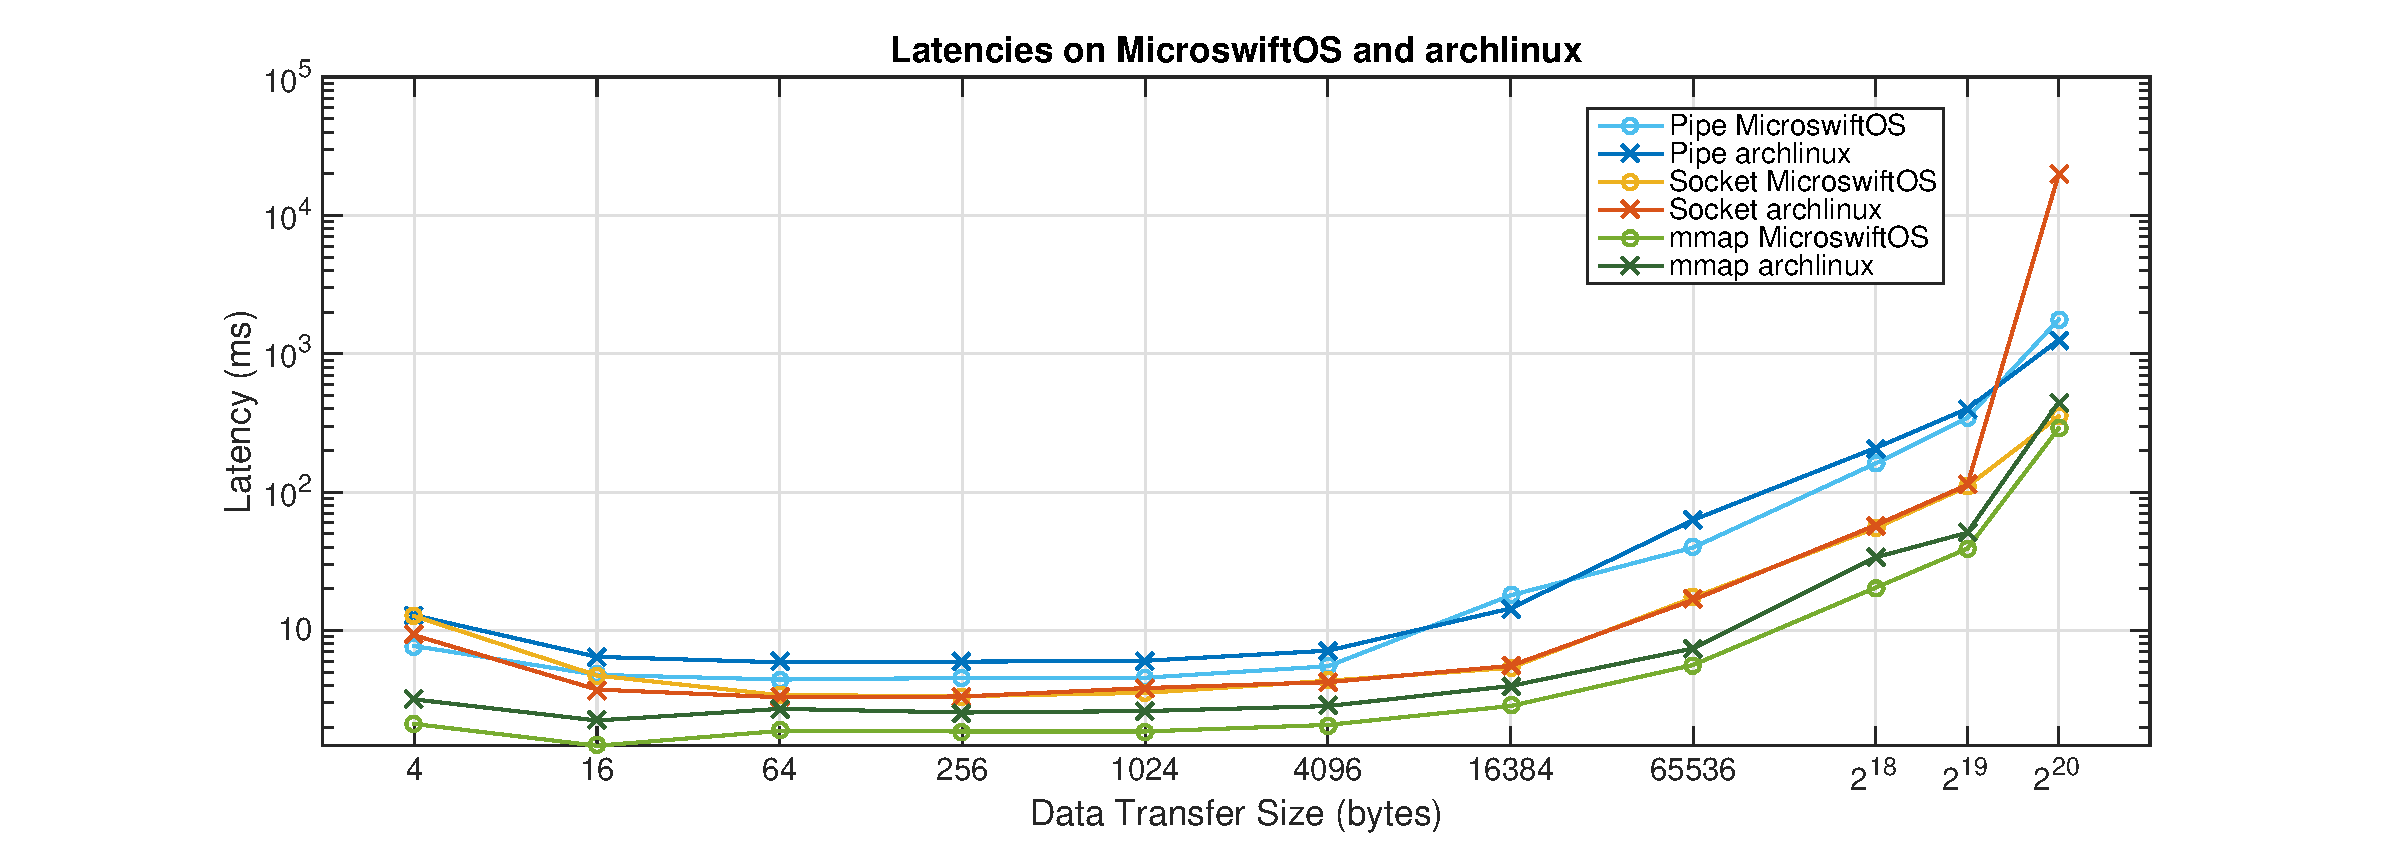
\epsfig{file=latencies.eps, width=6.8in}
\caption{Latencies for various IPC methods on MicroswiftOS and archlinux}
\label{figure:latency}
\end{figure*}

\begin{figure*}[!htb]
\centering
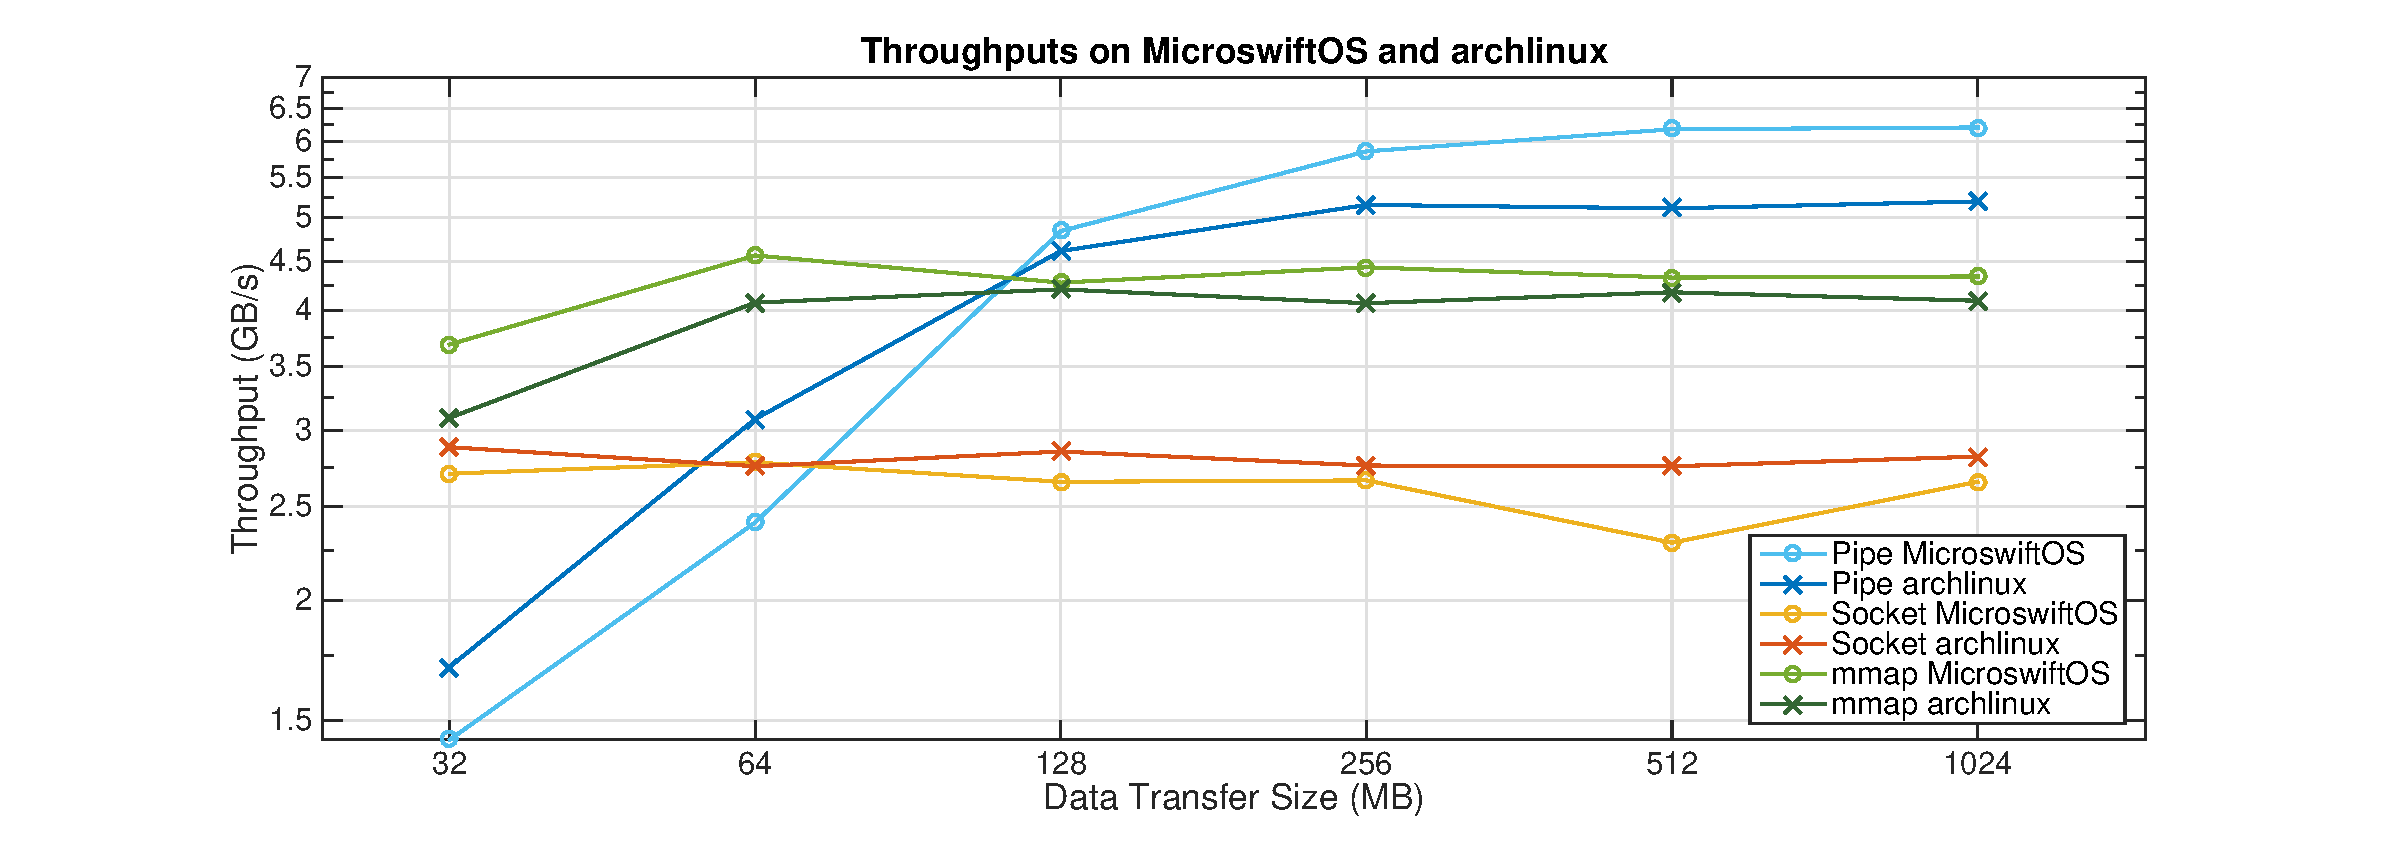
\epsfig{file=throughput.eps, width=6.8in}
\caption{Throughputs for various IPC methods on MicroswiftOS and archlinux}
\label{figure:throughput}
\end{figure*}

\subsection{System Size}
The disk spaces occupied by all MicroswiftOS files were about $900$MB, compared to $1.2$GB of a newly installed Archlinux. Note that we also included debug symbols of the linux kernel and gcc so as to make diagnosis easier. If debug symbols were removed, the size would be further smaller.


\section{Related Works}
\label{sec:related}
Kernel design for cloud computing is not a new yet very flourishing field. \cite{fox2009above} is a good introductory survey to cloud computing and it listed 10 big problems in this field. Though many problems have been attempted, more problems are rising over the horizon in the past few years. Kernel minimization does not only draw constant attention from academia, industrial world and computer amateurs also get involved in various communities. Here we list some recent research and projects that inspires our work. 
\subsection{Minimizing Kernel: Related Research}

The Nonkernel, introduced in \cite{ben2013nonkernel}, is a kernel design in which hardware resources are exposed to applications directly to reduce kernel booting time and to boost up parallelism and thus throughput. The Nonkernel does three things: 1) machine booting, 2) resource acquisition, and 3) application isolation. Machine booting is an intrinsic requirement of the kernel, and thus should be preserved. Resource acquisition is the management of hardware resources. Specifically, in a cloud computing environment, such mechanism must be provided and the kernel is in charge of resource arbitration. Finally application isolation is to guarantee that no applications should interfere with each other when accessing the same hardware resources. The Nonkernel provides an IPC mechanism that does not involve kernel. It is worth noting that traditional work such as processing scheduling and memory management are no longer the focus of a kernel design in a cloud computing. Nonkernel provides us with reference of cutting down a full-size kernel, yet there is no actual implementation. One major difference is that nonkernel serves as a "supervisor" in cloud computing, while our project aims to build a guest operating system.

Libra \cite{ammons2007libra} is the first operating system that specifically designed for JVM. It borrows the approach similar to exokernel, but avoids the problem of exokernel and reduces the cost of both developing a libOS and administering new partitions. With the use of a hypervisor, applications can use privileged execution modes and instructions, which enables optimizations and eases migration. In our projects we adopted the understanding an OS kernel as many functional parts, and may refer to the approach in this paper.

\subsection{Linux Kernel : Methodology, Tools and Tips from Industry}
Industrial world and computer amateurs share valuable experiences on that exploration to reduce boot time. The fastest boot time ever seen is within five seconds \cite{LPC} measured by Bootchart\cite{Bootchart} - Arjan van de Ven managed to boost Fedora 9 on an Asus EEE PC in five seconds, almost 90\% reduction in booting time compared to 45 seconds baseline. We find their approach inspiring for our project. Bootchart might be a useful tool for our project, though the last update was back in 2005.
Kernel booting consists of three phases: first Readahead module would read blocks of necessary modules from disk so that are cached in the memory, which will reduce cache miss and page fault during booting. Second, it goes along the critical path from filesystem checking to desktop displaying. Third step is hardware abstraction using HAL. These three phases start in sequential order but are running concurrently, and special arrangement has set up to achieve efficient CPU and disk utilization.

To extract basic components in an operating system and get rid of unnecessary ones is no easy task. It usually follows "trial and error" methodology that requires lots of labor and time. In \cite{gong2010characteristics}, basic OS requirements are defined and elaborated in a cloud computing context. For our project, we used this paper as a reference to set up the minimal feature set for our kernel design.

Mirage in \cite{madhavapeddy2010turning} is a specialized software stack designed for cloud use. Mirage is directly on top of the cloud hypervisor, and it entirely replaces the OS, user processes, runtimes, threads, and let applications directly run on Mirage. The advantages of efficiency, security, simplicity and easy deployment come from the characteristic of Mirage that it focus on the domain of I/O intensive cloud servers thus make it possible to specialize the stack. With the lack of OS and other standard software components of a computer, Mirage cannot run general-purpose applications, but can only be used for specialized applications like web servers. On the contrary, what we are trying to build is a general-purpose OS kernel that can run current applications on it without making any extra modifications.


\section{Future Work}
\label{sec:future}
One of the obstacles we are tackling is finding the symbols for the anonymous memory addresses we got in the perf report. We have tried the following tools and methods to solve the problem, but so far have not found a working solution:
\begin{enumerate}[(1)]
\item
Using pmap to gather information about the UML address space.
\item
Using objdump, nm and readelf to list symbols in an object file.
\item
Using gprof for sampling.
\end{enumerate}
For future research, we plan to try using gdb to set breakpoints to find out the commands corresponding to the memory addresses, and recover the missing symbols in the two flame graphs. From here we expect to gain more in depth understanding of the events and functions called during OS boot-up. Then we are able to find out the functions that take large portion of the booting time, look into the their implementations and examine optimization possibilities.


\section{Acknowledgement}
We would like to thank Michael Swift, Sanketh Nalli and Zhaoyu Luo for their helpful advices and comments. 


\section{Appendix A}
A summary of kernel configurations used in MicroswiftOS.
\begin{enumerate}
\item
Kernel hacking
	All supports in kernel hacking category could be disabled. Once our kernel is successfully set up for cloud computing, kernel hacking support could be minimized.
\item
Library routines
	All functions and algorithms can be disabled except mandatory ones such as CRC 16 functions, and CRC32/CRC32c functions.
\item
Cryptographic API
	All cryptographic functions could be disabled except mandatory ones such as CSC32c and AES cipher algorithms. The following two are supported by default kernel but could also be eliminated.
\begin{itemize}
\item
Hardware crypto devices
\item
Pseudo Random Number Generation for Cryptographic modules
\end{itemize}
\item
Security Options
	Default security configurations include networking support and cryptographic API. We leave this unchanged as we need to preserve networking related services.
\item
File System
	Our operating system uses ext4 file system we disabled support for following file systems.
\begin{itemize}
\item
Reiserfs support
\item
Miscellaneous filesystems
\item
Network file system
\end{itemize}
Along with disabled file systems we find two features that could also be disabled.
\begin{itemize}
\item
Native language support
\item
Dnotify support
\end{itemize}
Inotify support for userspace could not be removed from the kernel. Experiment shows that external storage devices could not be successfully unlicked and unmounted without inotify support.
\item
Networking support
	Default configurations for networking services include sockets, TCP/IP protocol stack. We leave this portion unchanged.
\item
Device Drivers
	Block devices and network devices are still supported by default. Sound card support is mandatory. IOMMU hardware support could be disabled. Everything else is disabled by default.
\item
Enable loadable module support
	This category of functionalities can be removed from the kernel. Loadable modules significantly reduce system speed and is not suitable for cloud use.
\item
General Setup
	This section includes a lot of configurations which are not tested yet. We have identified the following features that could be removed.
	\begin{itemize}
	\item
Automatically append version information to the version string
\item
\item Support for paging of anonymous memory (swap)
\item System V IPC
\item Optimize for size
\item Enable deprecated sysfs features to support old userspace tools
\item POSIX message queues
\item Timer subsystem (all items in it)
\item Enable access to .config through /proc/config.gz
\item Kernel .config support
\item Control group support
\end{itemize}
We could disable following features but we recognize that disabling will not necessarily reduce the boot time, hence we leave them as default.
\begin{itemize}
\item Disable heap randomization
\item Namespace support
\item BSD process accounting(in CPU/Task time and stats accounting)
\end{itemize}
\end{enumerate}


\section{Appendix B}

This section explains how test data were generated.
To test the max flow algorithm, we first generate a directed random with $100$ vertices, with each possible directed edge having a chance of $.1$ to appear.
Then we associate each edge with a uniformly randomly chosen capacity from the integers in $0..10$.
At last, two different vertices $s$ (source) and $t$ (sink) are randomly selected.
We generated $10$ such random networks to test the correctness of the maxflow algorithm.

To test the Gaussian-Jordan elimination algorithm, we generated a $100$-by-$100$ random matrix and a $100$-dimensional random vector.
Each entry of the matrix and the vector is chosen uniformly at random from real numbers in $[0,1]$.
Floating point tolerance has been set to $10^{-8}$, which means two matrices are considered equal if their dimensions match and the absolute difference between each corresponding entry is less than $10^{-8}$.

The simplex solver will try to optimize the following problem: maximize $c^T x$ subject to $Ax \leq b$ and $x \geq 0$, where $A$, $b$, $c$ are matrices and vectors of correct dimensions, and $x$ is the solution.
To test the correctness of the simplex algorithm, we pick the dimensions of the matrices as follows: $A$ $50$-by-$30$, $b$ $50$-by-$1$, $c$ $30$-by-$1$.
All entries in $A$, $b$, $c$ are chosen uniformly at random from real numbers in $[0,1]$.
Floating point tolerance has been set to $10^{-8}$.


\section{Appendix C}
This section includes two flame charts Figure \ref{fig:flame0} and Figure \ref{fig:flame1}. (See next 2 pages)
\begin{figure*}[!htb]
\centering
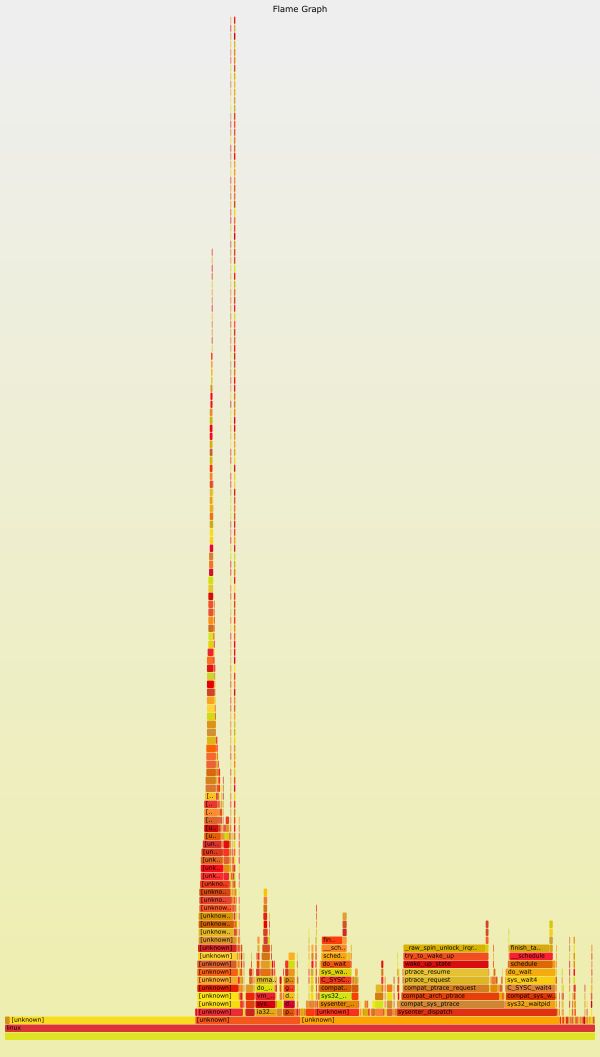
\includegraphics[width=5in]{0.png}
\caption{\label{fig:flame0}Flame chart for default configuration}
\end{figure*}

\begin{figure*}[!htb]
\centering
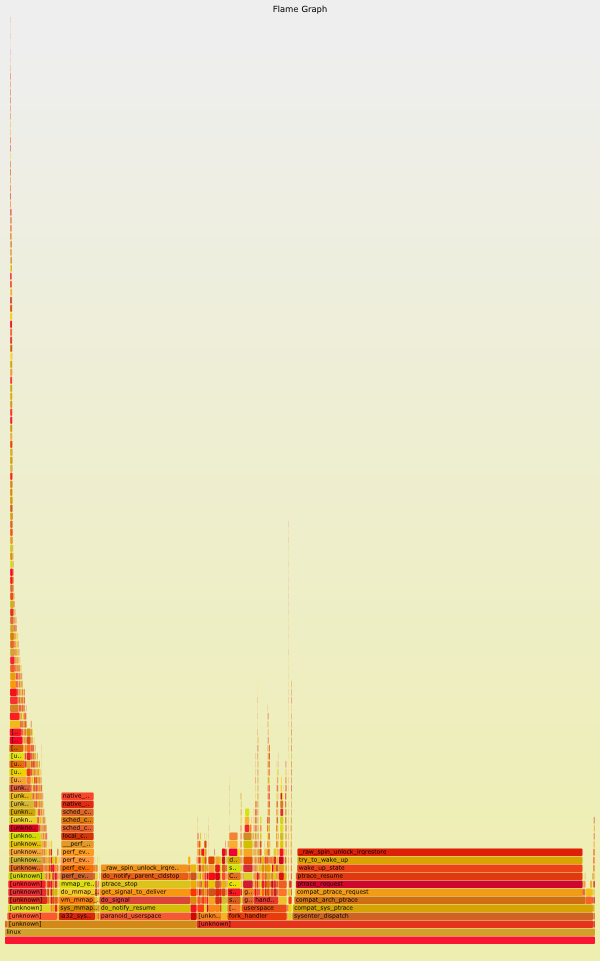
\includegraphics[width=5.5in]{1.png}
\caption{\label{fig:flame1}Flame chart for optimized configuration}
\end{figure*}

\section{Appendix D}
Table \ref{tab:1} is a list of software installed on MicroswiftOS.

\begin{table*}[!htb]
\centering
\caption{\label{tab:1}List of softwares installed on MicroswiftOS}
\begin{tabular}{|c|c|c|}
\hline
Glibc-2.21  & Zlib-1.2.8 & Binutils-2.25 \\
\hline
 Man-DB-2.7.1 & GMP-6.0.0a  & MPFR-3.1.2 \\
\hline
MPC-1.0.2  & GCC-4.9.2  & Bzip2-1.0.6 \\
\hline
 Vim-7.4 & Pkg-config-0.28  & Acl-2.2.52 \\
\hline
Libcap-2.24 &  Sed-4.2.2 & Shadow-4.2.1 \\
\hline
Patch-2.7.4 & Psmisc-22.21 & Procps-ng-3.3.10 \\
\hline
E2fsprogs-1.42.12 & Coreutils-8.23 & Iana-Etc-2.30 \\
\hline 
Sysvinit-2.88dsf& M4-1.4.17 &  Flex-2.5.39 \\
\hline
Bison-3.0.4 &  Grep-2.21 & Readline-6.3 \\
\hline
Eudev-2.1.1 &  Bash-4.3.30 & Libtool-2.4.6 \\
\hline
GDBM-1.11 & Inetutils-1.9.2 &  Autoconf-2.69 \\
\hline
 Tar-1.28& Automake-1.15 & Diffutils-3.3 \\
\hline
Findutils-4.4.2 & Gettext-0.19.4 & Gperf-3.0.4 \\
\hline
Util-linux-2.26 & Xz-5.2.0 & GRUB-2.02~beta2 \\
\hline
Less-458 &  Gzip-1.6 & IPRoute2-3.19.0 \\
\hline
Sysklogd-1.5.1 & Make-4.1 &  \\
\hline
\end{tabular}
\end{table*}


% \bibliographystyle{abbrv}
\bibliographystyle{plain}
\bibliography{references}

% \end{multicols}
\end{document}

% \begin{table}[!htb]
% \centering
% \begin{tabular}{|c||c|c|c|}
% \hline
% \multirow{3}{*}{\textbf{Benchmark}} & \textbf{Additional} & \textbf{Total} &\multirow{3}{*}{\textbf{Percentage}}\\ 
% &\textbf{Memory} &\textbf{Memory}&\\
% &\textbf{Accesses} &\textbf{Accesses} &\\ \hline \hline
% aster & 175481 & 2404970 & 0.0730\\ \hline 
% bzip2 & 1067380 & 9188892 & 0.1162\\ \hline 
% lbm   & 130990 & 5003775 & 0.0262\\ \hline 
% libquantum   & 54796 & 3092800 & 0.0177\\ \hline 
% milc  & 136746 & 5575859 & 0.0245\\ \hline 
% omnetpp  & 107165 & 287076 & 0.3733\\ \hline 
% \textbf{Average} & \textbf{-} &\textbf{- } &\textbf{0.1051}\\ \hline
% \end{tabular}
% \caption{Additional memory accesses for storing reuse data in a 1MB L2 reuse cache during a simulation period of 300M instructions}
% \label{table:additionalaccess}
% \end{table}

% \begin{figure}[!htb]
% \centering
% \epsfig{file=ReuseStruct.eps, height =2in, width =2in}
% \caption{Structure of our implementation for the reuse cache}
% \label{reuse:struct}
% \end{figure}

% \begin{table}[!htb]
% \centering
% \begin{tabular}{|c||c|c|c|}
% \hline
% \multirow{3}{*}{\textbf{benchmark}} & \textbf{memory} & \textbf{total} & \multirow{3}{*}{\textbf{percentage}}\\
% &\textbf{write} &\textbf{memory} &\\
% & \textbf{miss times} & \textbf{access times} & \\ \hline\hline
% bzip2 & 778893 & 16791412 & 0.0464\\ \hline 
% aster & 83555 & 4487131 & 0.0186\\ \hline 
% libquantum & 35243 & 6091860 & 0.0058\\ \hline 
% lbm & 72942 & 9862259 & 0.0074\\ \hline 
% milc & 69407 & 10820712 & 0.0064\\ \hline 
% omnetpp & 83508 & 416317 & 0.2006 \\ \hline

% \textbf{Average} &\textbf{-} &\textbf{-} &\textbf{0.0475}\\

% \hline
% \end{tabular}
% \caption{Memory write miss times in a 1MB reuse cache during a simulation period of 300M instructions}
% \label{table:writemiss}
% \end{table}



% \begin{table}[!htb]
% \centering
% \begin{tabular}{|l||r|}
% \hline
% L1 data cache size & 64KB\\
% \hline
% L1 data cache associativity & 4-way\\
% \hline
% L1 instruction cache size & 32KB\\
% \hline
% L1 instruction cache associativity & 4-way\\
% \hline
% L2 cache size & 1MB\\
% \hline
% L2 cache associativity & 8-way\\
% \hline
% Cache line size & 64B\\
% \hline
% Single memory size & 512 MB\\
% \hline
% \end{tabular}
% \caption{System configurations for baseline performance}
% \label{table:baselineconfig}
% \end{table}


% \begin{figure*}[!htb]
% \centering
% \epsfig{file=rc248.eps, width=7in}
% \caption{Relative performace of reuse cache under varying data array sizes. The data array sizes for ratio 2, 4, 8 are 512KB, 256KB, 128KB, respectively.}
% \label{fig:rc248}
% \end{figure*}



% \begin{figure}[!htb]
% \centering
% \epsfig{file=bzip2live.eps, width=3.4in}
% \caption{bzip2 percentage of live lines during execution of workload. Sampling is once per 100K data accesses.}
% \label{fig:bzip2live}
% \end{figure}

% \begin{figure*}[!htb]
% \centering
% \epsfig{file=addarray.eps, width=7in}
% \caption{Relative performace of reuse cache under varying additional block array sizes. The additional block array sizes for ratio 16, 32, 64 are 64KB, 32KB, 16KB, respectively. No additional block array means a regular reuse cache design. All statistics are obtained when reuse cache tag/data ratio is 2.}
% \label{fig:addarray}
% \end{figure*}


% \begin{table*}[!htb]
% \centering
% \begin{tabular}{|c||c|c|c|c|c|c|}
% \hline
% \multirow{2}{*}{\textbf{Benchmark}} & 
% \multicolumn{2}{c|}{\textbf{Ratio 2}} & \multicolumn{2}{c}{\textbf{Ratio 4}} & \multicolumn{2}{|c|}{\textbf{Ratio 8}}\\
% \cline{2-7}
% & \textbf{Speedup} & \textbf{Miss Rate} & \textbf{Speedup} & \textbf{Miss Rate} & \textbf{Speedup} & \textbf{Miss Rate} \\ \hline
% astar & 0.983 & 1.046 & 0.984 & 1.042 & 0.972 & 1.069\\ \hline 
% bwaves & 0.923 & 1.064 & 0.935 & 1.079 & 0.945 & 1.067\\ \hline 
% bzip2 & 0.858 & 1.114 & 0.833 & 1.112 & 0.820 & 1.154\\ \hline 
% lbm & 0.966 & 1.010 & 0.974 & 0.981 & 0.973 & 0.982\\ \hline 
% libquantum & 0.957 & 1.015 & 0.964 & 1.020 & 0.979 & 1.045\\ \hline 
% mcf & 0.876 & 1.700 & 0.833 & 2.030 & 0.796 & 2.383\\ \hline 
% milc & 0.988 & 1.016 & 0.989 & 1.021 & 0.992 & 1.014\\ \hline 
% omnetpp & 0.973 & 1.689 & 0.940 & 3.202 & 0.848 & 8.054\\ \hline 
% \textbf{Average} & \textbf{0.939} &\textbf{1.070} &\textbf{0.930} & \textbf{1.091} &\textbf{0.913} &\textbf{1.148}\\ \hline
% \end{tabular}
% \caption{Speedup and miss rate of workloads relative to baseline. Ths miss rate is a relative ratio compared with baseline miss rate.}
% \label{table:missrate}
% \end{table*}
